\chapter{Design of Quadrotor}\label{design}

In this chapter, the system architecture is presented, including the software and hardware configurations, specifications of the UAV platform and details of sensors.

\section{Hardware architecture}\label{hardware}

\begin{figure}[ht]
  \centering
  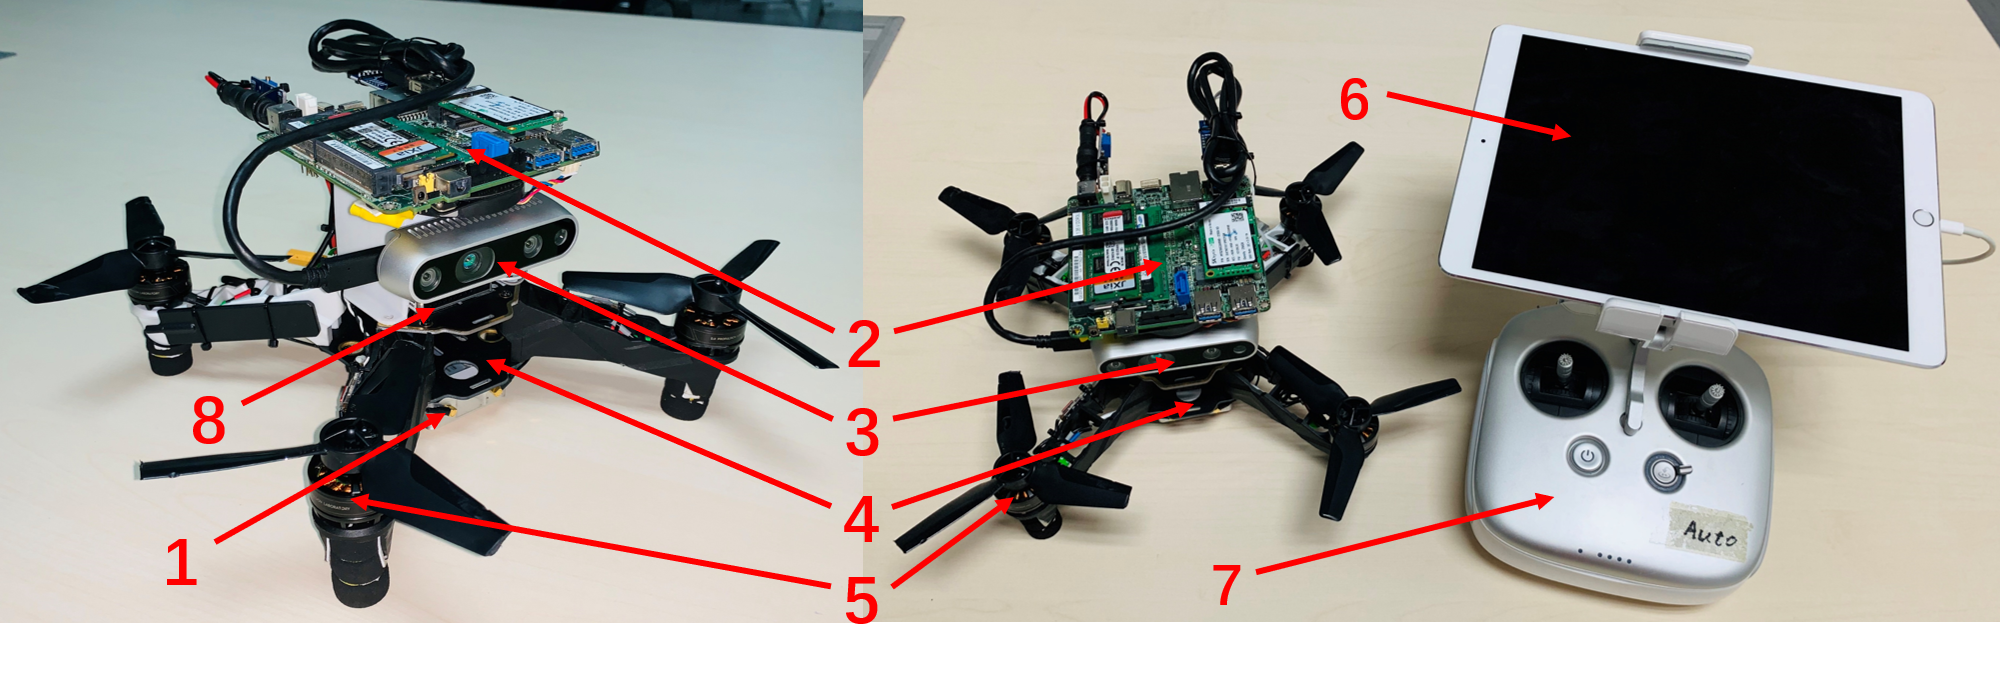
\includegraphics[width=1.0\textwidth]{figure/chaser_intro.eps}
  \caption{Chaser quadrotor and remote controller panel: (1) Lightbridge 2 receiver; (2) Intel NUC mini computer; (3) 4S LiPo Batter; (4) Intel Realsense camera; (5) DJI snail motor; (6) iPad Live streaming panel; (7) DJI Lightbridge 2 remote controller; (8) DJI N3 flight controller}
  \label{fig:quadrotor_controller}
\end{figure}

The hardware of UAV platform includes one chaser quadrotor, one target quadrotor and their remote controllers (RCs) as shown in Figure~\ref{fig:quadrotor_controller},~\ref{fig:target_uav}. The quadrotor is first controlled by the RC to take off, then the control authority is switched to on-board mini computer by RC to achieve autonomous driving. The RC has higher control authority than on-board computer that human operator could prevent quadrotor from fatal errors by switching control priority back to RC.

\begin{figure}[ht]
  \centering
  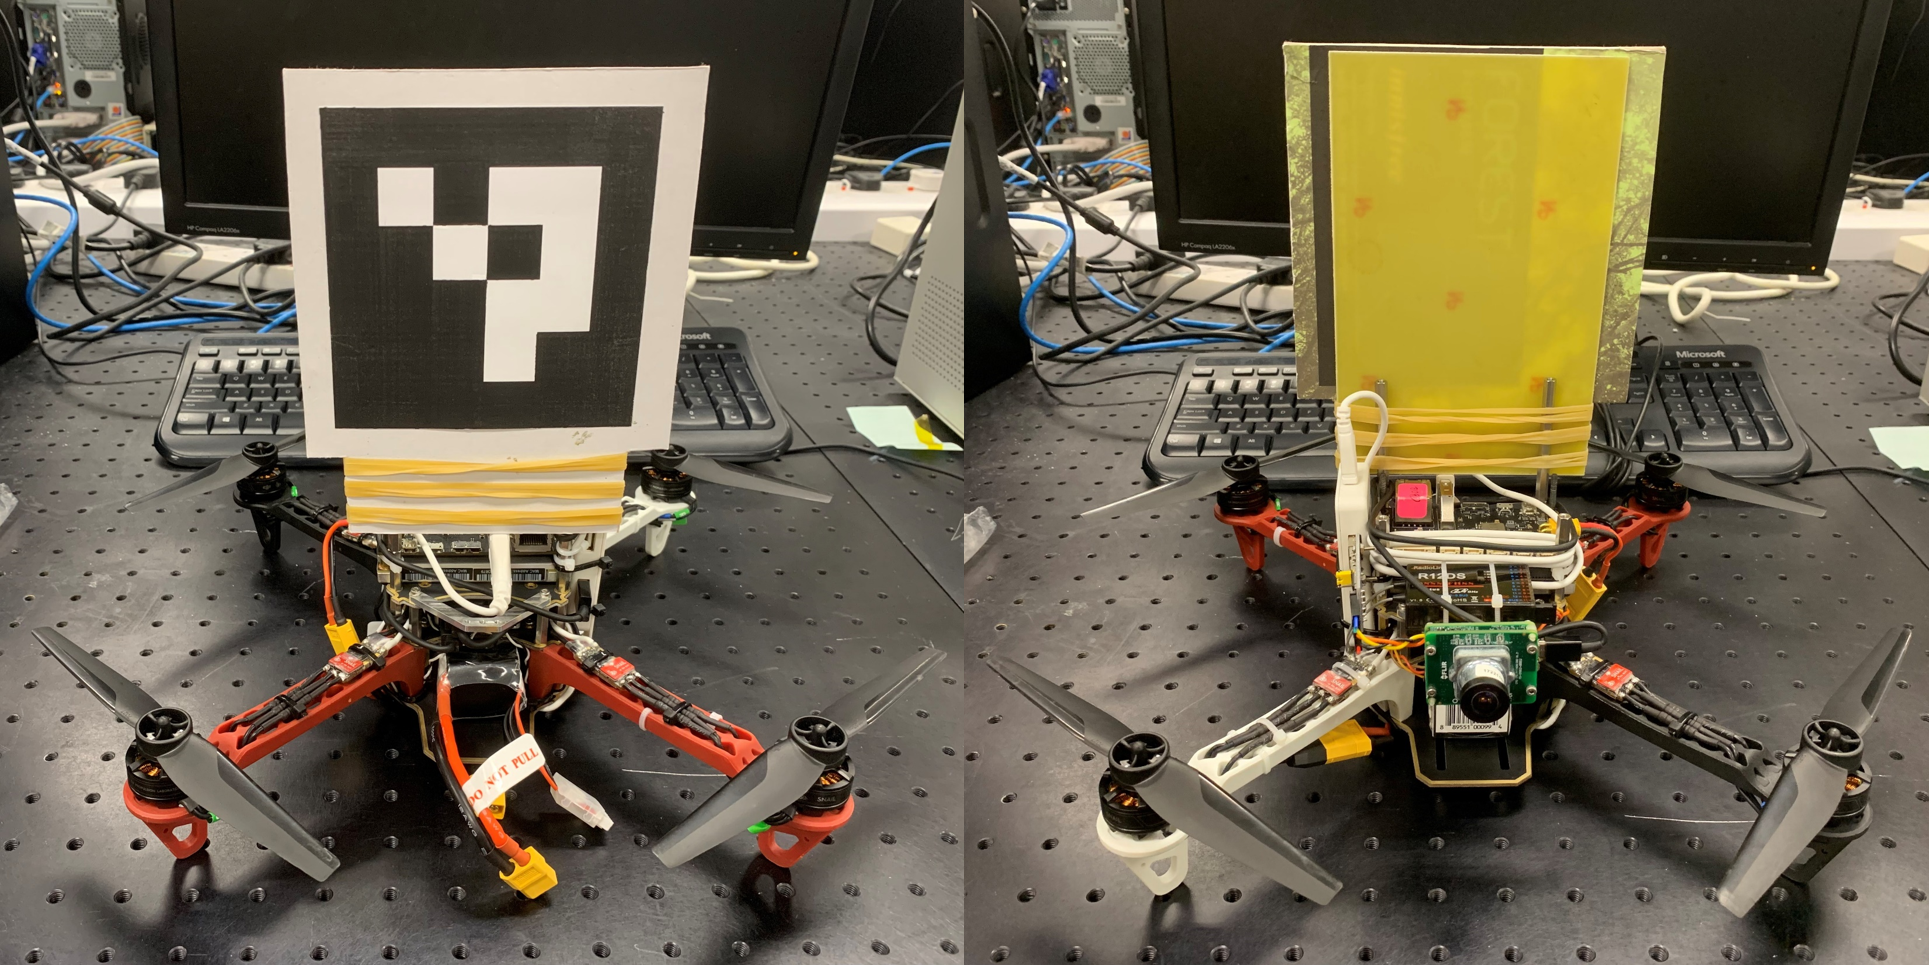
\includegraphics[width=1.0\textwidth]{figure/target_uav.eps}
  \caption{target quadrotor. left: back; right: front}
  \label{fig:target_uav}
\end{figure}

\begin{table}[htb]
  \centering
 \linespread{1.7}{ {\footnotesize
\vspace{2em}
  \begin{tabular}{ccc}
  \hline
\noalign{\smallskip}
  \textbf{Component} & \textbf{Weight(g)} & \textbf{Power(W)}\\
\noalign{\smallskip}
  \hline
  Intel NUC i5 mini computer & 125 & 15(avg) \\
  Intel Realsense D435i camera & 272 & 2.5(avg) \\
  DJI N3 flight controller & 92 & 3.3(avg)/5(peak) \\
  DJI Lightbridge 2 receiver & 70 &  7.8(avg)\\
\noalign{\smallskip}
  \hline
  \end{tabular}
  }}
  \caption{Weight and power consumption of components on the quadrotor}
  \label{tb:weight_power}
\end{table}

\begin{figure}[ht]
  \centering
  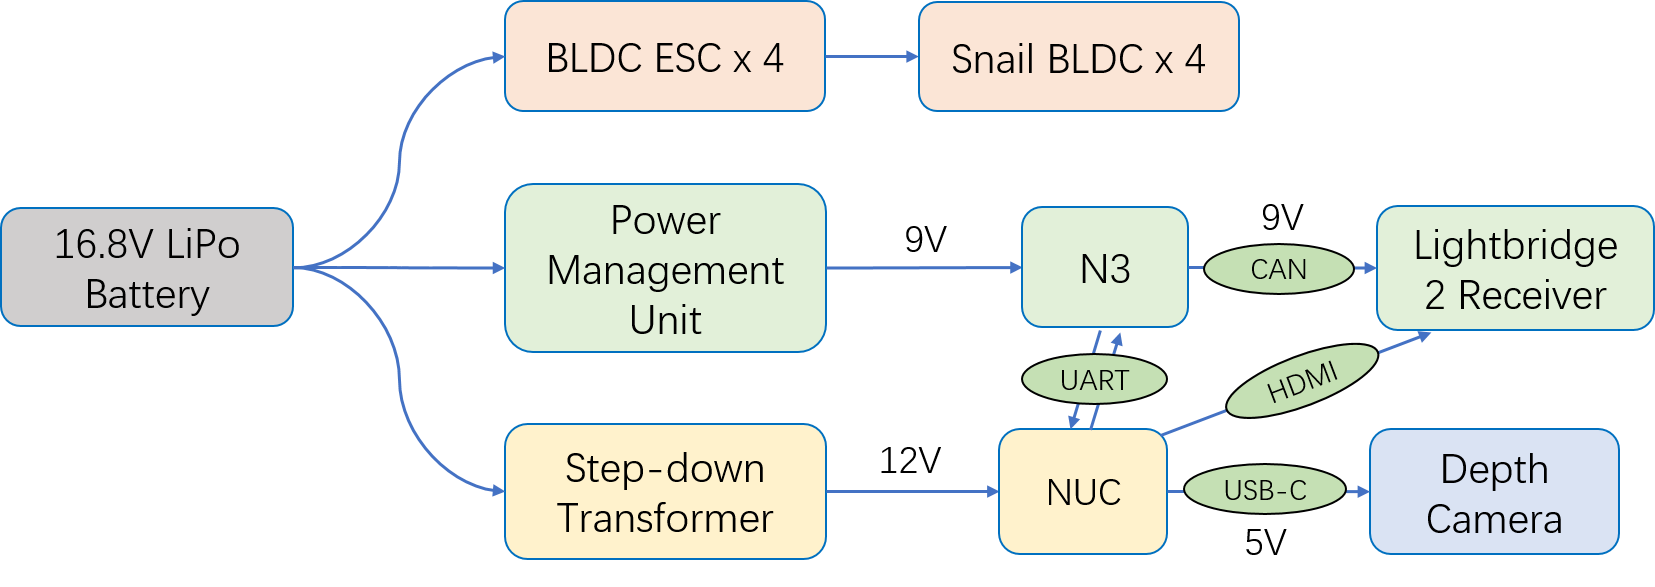
\includegraphics[width=1.0\textwidth]{figure/power_system.eps}
  \caption{On-board power systems}
  \label{fig:power_systems}
\end{figure}

The quadrotor frame consists of the mechanical construction, motors, propellers and the power supply module. Q250 is chosen as the chaser quadrotor frame for its compact size, firm material and the flexibility in maneuvering in cluttered environment. DJI snail BLDC motors and 5 inch 3-blade propellers are mounted for their racing optimized propulsion system and rapid response time. 4S LiPo battery is selected for on-board power supply for its 16.8 V output, 4200 mAh capacity and rechargeable property. The detailed chaser power supply system is illustrated in Figure~\ref{fig:power_systems}. The total weight including the battery is 1.25 kg and the diagonal distance is 25 cm. We use Intel NUC i5 mini computer as our chaser quadrotor main on-board computing resource for both frontend processing and backend optimization. We choose Intel Realsense Depth camera D435i as the forward looking camera for chaser quadrotor's perception and target recognition purposes. It is outfitted with a stereo global shutter camera, with resolution up to 1920x1080 pixels, frame rate up to 90 fps and direct depth map output. More details about on-board components can be found in Table~\ref{tb:weight_power}.

The overall system stability is more emphasized than flexibility on target quadrotor, where F330 frame with diagonal distance of 33 cm, snail BLDC motors and 7 inch propellers are mounted. The demand for computation and perception capability on target quadrotor is lower than the chaser, as its flight path is either controlled by human operator or pre-defined in its on-board computer. In this scenario, NVIDIA Jetson TX2 and Machine Vision Point Grey monocular camera are mounted respectively. DJI N3 flight controller is selected for both chaser and target quadrotor, due to its high quality built-in IMU sensor and compatibility with DJI Lightbridge 2 for live streaming.

\section{Software architecture}\label{software}

\begin{figure}[ht]
  \centering
  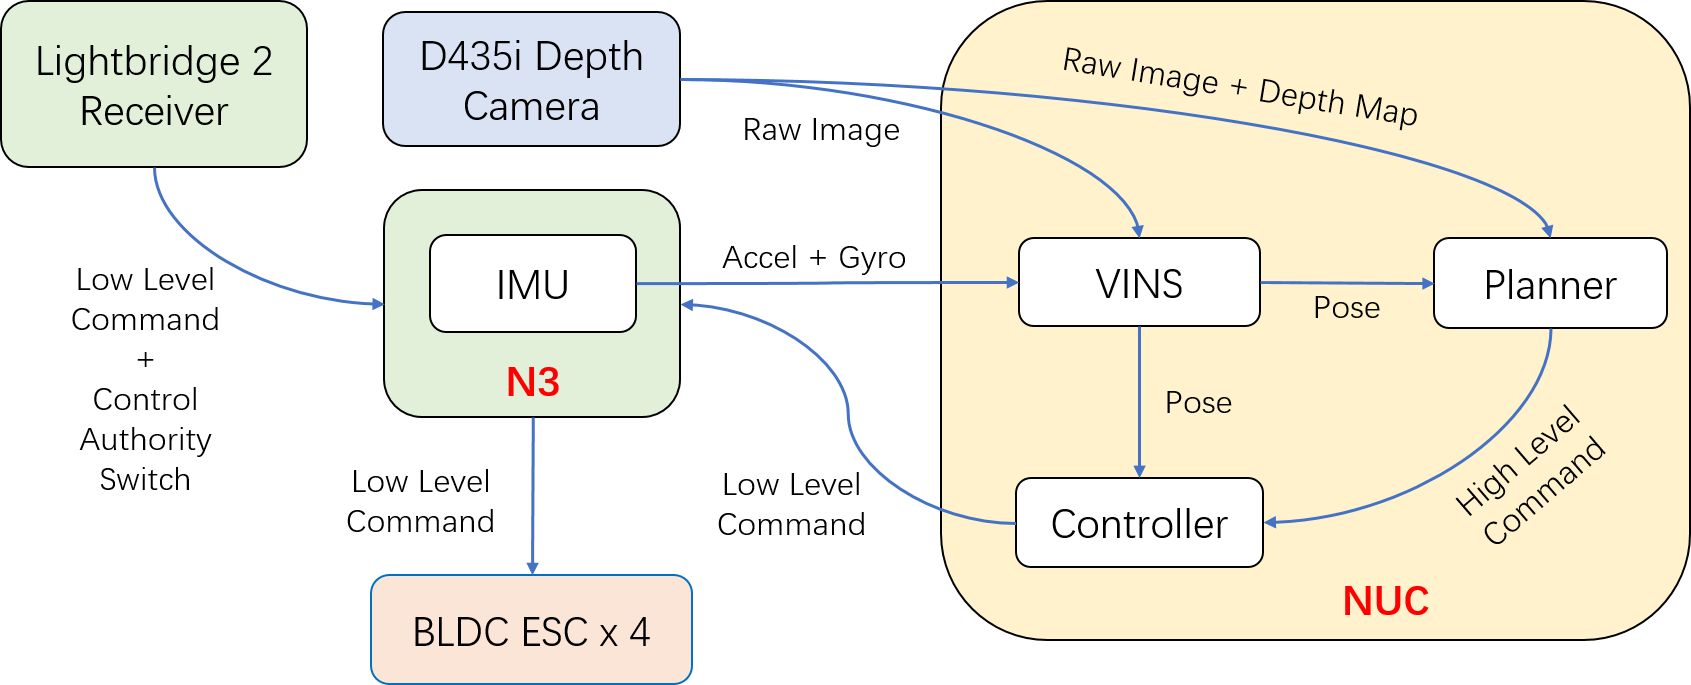
\includegraphics[width=1.0\textwidth]{figure/system_diagram.eps}
  \caption{Software architecture}
  \label{fig:software_architecture}
\end{figure}

The software architecture is shown in Figure~\ref{fig:software_architecture}. On chaser's mini i5 computer, 100 Hz IMU measurements and 10 Hz grey scale image data are fused in the visual-inertial state estimator~\cite{VINS} to obtain UAV self position and orientation. Unique aruco code~\cite{Aruco} is attached on target UAV for relative pose estimation and motion prediction. Using predicted target future motion and current chaser pose, a smooth trajectory for chaser UAV is planned and executed with the attitude and thrust control interface in DJI N3 flight controller. Unlike many existing systems that rely on downward facing camera, ultrasonic sensor or LIDAR for sensing, our system only utilize one forward looking camera. We show through both indoor and outdoor experiments that our minimal sensing setup is sufficient for autonomous tracking of an aerial target.

We have also utilized DJI Lightbridge 2 for remote debugging and monitoring. The Lightbridge 2 transforms mini computer's desktop stream to iPad Pro for visualization, including current chaser's pose and live image processing output. This enables us to remotely manipulate the on-board computer while the quadrotor is in the air.

\newpage
